\hspace{\parindent}Several test types have been done for the app. Most of the testing was done during the app development, so further Unit testing was reduced as most of it was done before.

\subsection{Unit testing}
\hspace{\parindent}The main part of the testing was done by unit testing.
Four major unit tests have been created that test functionalities of the main parts of the app. Each main test has several subtests. For code conciseness purposes main tests are not a set of small tests, but just one large test that tests multiple different parts of the subsystem.\\ \\

When counting the total number of tested subcomponents, we have done approximately XY small tests, separated into four major groups, which are:
\begin{itemize}
\item Login tests (7)
\item Trip Creation Activity tests (12)
\item Navigation tests (6)
\item Map screen tests (5)
\end{itemize}

These tests are now going to be showcased and presented.
\subsubsection{Login unit testing}
The tests done for login testing:
\begin{itemize}
\item Inputting username
\item Inputting password
\item Testing login
\item Testing login with false authentication
\item Testing login with correct authentication
\item Logging in with Google Account
\item Logging in with Facebook acocunt
\end{itemize}

The code:
\begin{verbatim}
@RunWith(AndroidJUnit4::class)
class LoginTest : TestCase() {

    @OptIn(
        ExperimentalFoundationApi::class,
    kotlinx.coroutines.ExperimentalCoroutinesApi::class,
        androidx.compose.animation.ExperimentalAnimationApi::class,
        androidx.compose.material.ExperimentalMaterialApi::class
    )
    @get:Rule
    val composeTestRule = createAndroidComposeRule<LoginActivity>()
    @OptIn(
        ExperimentalCoroutinesApi::class,
        androidx.compose.foundation.ExperimentalFoundationApi::class,
        androidx.compose.animation.ExperimentalAnimationApi::class,
        androidx.compose.material.ExperimentalMaterialApi::class
    )
    @Test
    fun checkLogin() {
        val login = composeTestRule.onNodeWithTag("login")
        val usr = composeTestRule.onNodeWithTag("username")
        val pwd = composeTestRule.onNodeWithTag("password")
            usr.performTextInput("vins@vins.com")
            pwd.performTextInput("vins")
            login.performClick()
        composeTestRule.onNode(hasText("Authentication failed"))
        assertFalse(composeTestRule.activity.isNewUser ?: false)
        pwd.performTextClearance()
        pwd.performTextInput("vinsvins")
        login.performClick()
        Thread.sleep(5000)
        getInstrumentation().runOnMainSync {
            val activity =
                ActivityLifecycleMonitorRegistry.getInstance().getActivitiesInStage(
                    Stage.RESUMED
                ).first()
            assertTrue(activity is MainActivity)
        }
    }
}

\end{verbatim}

\subsubsection{Trip creation activity unit testing}
The tests done for trip creation activity testing:
\begin{itemize}
\item Tests whether the trip can be created correctly.
\item The following elements of the trip creation screen are tested:
\item Inputting text to name field
\item Inputting text to description field
\item Inputting multiple tags
\item Searchig destinations with city name
\item Adding steps
\item Adding main destinations
\item Exiting without saving
\item Exiting with saving
\item Trying to save trip without filling all the required fields
\item Failing to save trip
\end{itemize}

\begin{verbatim}
-	@RunWith(AndroidJUnit4::class)
class TripCreationActivityTest : TestCase() {
    @get:Rule
    val composeTestRule = createAndroidComposeRule<TripCreationActivity>()
    @OptIn(ExperimentalTestApi::class)
    @Test
    fun create() {
        composeTestRule.onNodeWithTag("name").performTextInput("Nome")
        composeTestRule.onNodeWithTag("description").
        performTextInput("Description")
        val tag = composeTestRule.onNodeWithTag("tag")
        tag.performTextInput("tag1")
        tag.performTextInput(",")
        tag.performTextInput("tag2")
        tag.performTextInput(",")
        composeTestRule.onNodeWithTag("main").performClick()
        Thread.sleep(1000)
        composeTestRule.onNodeWithTag("searchText").
        performTextInput("verona")
        composeTestRule.onNodeWithTag("searchText").
        performImeAction()
        Thread.sleep(4000)
        composeTestRule.
        onAllNodes(hasText("Verona",true,true)).
        onFirst().assertExists()
        val addStep = composeTestRule.onAllNodesWithTag("add").onFirst()
        addStep.assertExists()
        addStep.performClick()
        val setMain = composeTestRule.onAllNodesWithTag("main").onFirst()
        setMain.assertExists()
        setMain.performClick()
        composeTestRule.onNodeWithTag("back").performClick()
        Thread.sleep(500)
        val nodes = composeTestRule.onAllNodes(hasText("verona",true,true))
        assertNotNull(nodes)
        nodes.assertCountEquals(2)
        composeTestRule.onNodeWithTag("confirm").performClick()
        Thread.sleep(2000)
        InstrumentationRegistry.getInstrumentation().runOnMainSync {
            val activity =
                ActivityLifecycleMonitorRegistry.getInstance().
            getActivitiesInStage(
                    Stage.DESTROYED
                ).first()

            assertTrue(activity is TripCreationActivity)

        }
    }
    
    @Test
    fun creationFailure() {
        for (i in 0..3) {
            if (i == 0)
                composeTestRule.onNodeWithTag("name").
            performTextInput("Nome")
            if (i == 1)
                composeTestRule.onNodeWithTag("description")
            .performTextInput("Description")
            if (i == 2) {
                val tag = composeTestRule.onNodeWithTag("tag")
                tag.performTextInput("tag1")
                tag.performTextInput(",")
                tag.performTextInput("tag2")
                tag.performTextInput(",")
            }
            if (i == 3) {
                composeTestRule.onNodeWithTag("main").performClick()
                Thread.sleep(1000)
                composeTestRule.onNodeWithTag("searchText").
                performTextInput("verona")
                composeTestRule.onNodeWithTag("searchText").
                performImeAction()
                Thread.sleep(4000)
                composeTestRule.onAllNodes(hasText("Verona", true, true)).onFirst().assertExists()
                val addStep = composeTestRule.onAllNodesWithTag("add").onFirst()
                addStep.assertExists()
                addStep.performClick()
                val setMain = composeTestRule.onAllNodesWithTag("main").onFirst()
                setMain.assertExists()
                setMain.performClick()
                composeTestRule.onNodeWithTag("back").performClick()
                Thread.sleep(500)
                val nodes = composeTestRule.onAllNodes(hasText("verona", true, true))
                assertNotNull(nodes)
                nodes.assertCountEquals(2)
            }
            composeTestRule.onNodeWithTag("confirm").performClick()
            Thread.sleep(1000)
            val text = composeTestRule.activity.getString(R.string.not_enough_info)
            if (i != 3)
                onView(withText(text)).check(matches(isDisplayed()))
            Thread.sleep(2000)
        }
    }
}

\end{verbatim}

\subsubsection{Navigation unit testing}
The tests done for trip creation activity testing:
\begin{itemize}
\item Navigation of the bottom tab
\item Navigation of home screen
\item Navigation of map screen
\item Navigation of trip screen
\item Navigation of explore screen
\item Navigation of profile screen
\end{itemize}

\begin{verbatim}
@RunWith(AndroidJUnit4::class)
class NavigationTest : TestCase() {
    @get:Rule
    val composeTestRule = createAndroidComposeRule<MainActivity>()

    @Test
    fun navigation() {
        for (i in 0..6) {
            composeTestRule.onNodeWithTag("tab" + nextInt(0, 4)).performClick()
            Thread.sleep(3000)
        }
        composeTestRule.onNodeWithTag("tab4").performClick()
        assertNotNull(composeTestRule.onNode(hasText("Astro",true,true)))
        composeTestRule.onAllNodesWithTag("positive").onFirst().performClick()
        Thread.sleep(2000)
        composeTestRule.onAllNodesWithTag("negative").onFirst().performClick()

        composeTestRule.onNodeWithTag("tab3").performClick()

        composeTestRule.onNodeWithTag("around").performClick()
        Thread.sleep(3000)
        getInstrumentation().runOnMainSync {


            val activity =
                ActivityLifecycleMonitorRegistry.getInstance().
                getActivitiesInStage(
                    Stage.RESUMED
                ).first()

            assertTrue(activity is AroundMeActivity) 
            // seems to not work in Debug test mode
            // works in release
        }
    }
}

\end{verbatim}
\subsubsection{Map screen unit testing}
The tests done for trip creation activity testing:
\begin{itemize}
\item Navigate to tab
\item Draw a polygon in the map tab
\item Retrieve results of the drawn polygon
\item Selection of the shown destination
\item Detail displaying of the destination
\end{itemize}
\begin{verbatim}
@RunWith(AndroidJUnit4::class)
class MapScreenTest : TestCase() {


    @get:Rule
    val composeTestRule = createAndroidComposeRule<MainActivity>()

    @OptIn(ExperimentalTestApi::class)
    @Test
    fun checkSelection() {
        composeTestRule.onNodeWithTag("tab1").performClick()
        Thread.sleep(1000)
        composeTestRule.onNodeWithTag("draw").performClick()
        Thread.sleep(1000)
        val device = UiDevice.getInstance(getInstrumentation())


        // It requires to disable animations by phone settings
        // + declare injection_event permission
        // For the release, this requirements have been turned off
        try {
            composeTestRule.onRoot().performGesture {
                down(Offset(50f,50f))
                moveBy(Offset(500f,500f))
                moveBy(Offset(500f,0f))
                moveBy(Offset(-500f,500f))
            }
            composeTestRule.onNodeWithTag("draw").performClick()
        }
        catch (e: Exception) {
            Log.e("TEST",e.localizedMessage)
        }
        val marker = device.findObject(UiSelector().descriptionContains("Venice"))
        marker.click()
    }

}

\end{verbatim}
\newpage
\subsection{Deep linking testing}
\hspace{\parindent}Deep linking testing has been done by providing the application with three different types of links - the correct type of link accepted by the application (schema, host, and attribute part are accepted), semi-correct type of link (schema and host are accepted, the attribute is not), and the correct link with false attribute value.\\ \\

For testing purposes, Android Debug Bridge (adb) and manual link clicking have been used. Here are the results of several tests done via adb:\\

\textbf{Test 1}
\begin{verbatim}
adb shell am start
>adb shell am start -W -a android.intent.action.VIEW
Starting: Intent { act=android.intent.action.VIEW }
Status: ok
LaunchState: COLD
Activity: android/com.android.internal.app.ResolverActivity
TotalTime: 457
WaitTime: 527
Complete
\end{verbatim}

\textbf{Test 2}
\begin{verbatim}
>adb shell am start -W -a 
android.intent.action.VIEW -d "https://polaris.travel.app/find/tripID"
Starting: Intent { act=android.intent.action.VIEW dat=https://polaris.travel.app/... }
Status: ok
LaunchState: WARM
Activity: android/com.android.internal.app.ResolverActivity
TotalTime: 251
WaitTime: 258
Complete
\end{verbatim}

\textbf{Test 3}
\begin{verbatim}
>adb shell am start -W -a 
android.intent.action.VIEW -d "https://polaris.travel.app/find/tripID"
Starting: Intent { act=android.intent.action.VIEW dat=https://polaris.travel.app/... }
Status: ok
LaunchState: COLD
Activity: web/android.default.webApp
TotalTime: 251
WaitTime: 258
\end{verbatim}

The tests that have correct deep links have opened the Polaris activity, while the link with incorrect link has opened the 
link directly in the browser.

\newpage
\subsection{Failure test}
We have done a process of a failure test when if comes to the app functioning in both online and offline mode. As the app features both states, it is important that the app works in offline mode properly even when there is no Internet connection, and that it restores to a proper flow once the Internet connection is present.\\

This is the following set of actions done for this test:
\begin{enumerate}
\item Shut down the server
\item Enter the app and navigate it with internet connection enabled
\item Check the app doesn't crash and gracefully alerts the user of the problem
\item Put the server up
\item Check everything is correctly received 
\item Change endpoint
\item Redo points 2. and 3.
\item Put the server in a inconsistent status of responses
\item Redo points 2. and 3.
\item Restore server in a consistent configuration
\item Disabling local connectivity (offline status)
\item Redo points 2. and 3.
\end{enumerate}
All of the tests regarding failure have been passed successfully.
\newpage
\subsection{Support of different devices}
\hspace{\parindent}The app has been tested on several different device types and screen sizes. The testing has been done either on real world devices or on the virtual devices, ranging from Android 8 to Android 11. The list of the devices the app has been tested is the following:
\begin{itemize}
\item Samsung Galaxy S6
\item Samsung Galaxy A50
\item Samsung Galaxy A51
\item Google Pixel 3a
\item Samsung Galaxy Tablet S5 (Tablet)
\item Google Nexus 7 (Tablet)
\item Google Pixel C (Tablet)
\end{itemize}

Here are a few screenshot examples of the same screen working on devices of two different sizes (phone and tablet):

\begin{figure}[!htb]
\centering
\begin{minipage}{.45\textwidth}
\centering
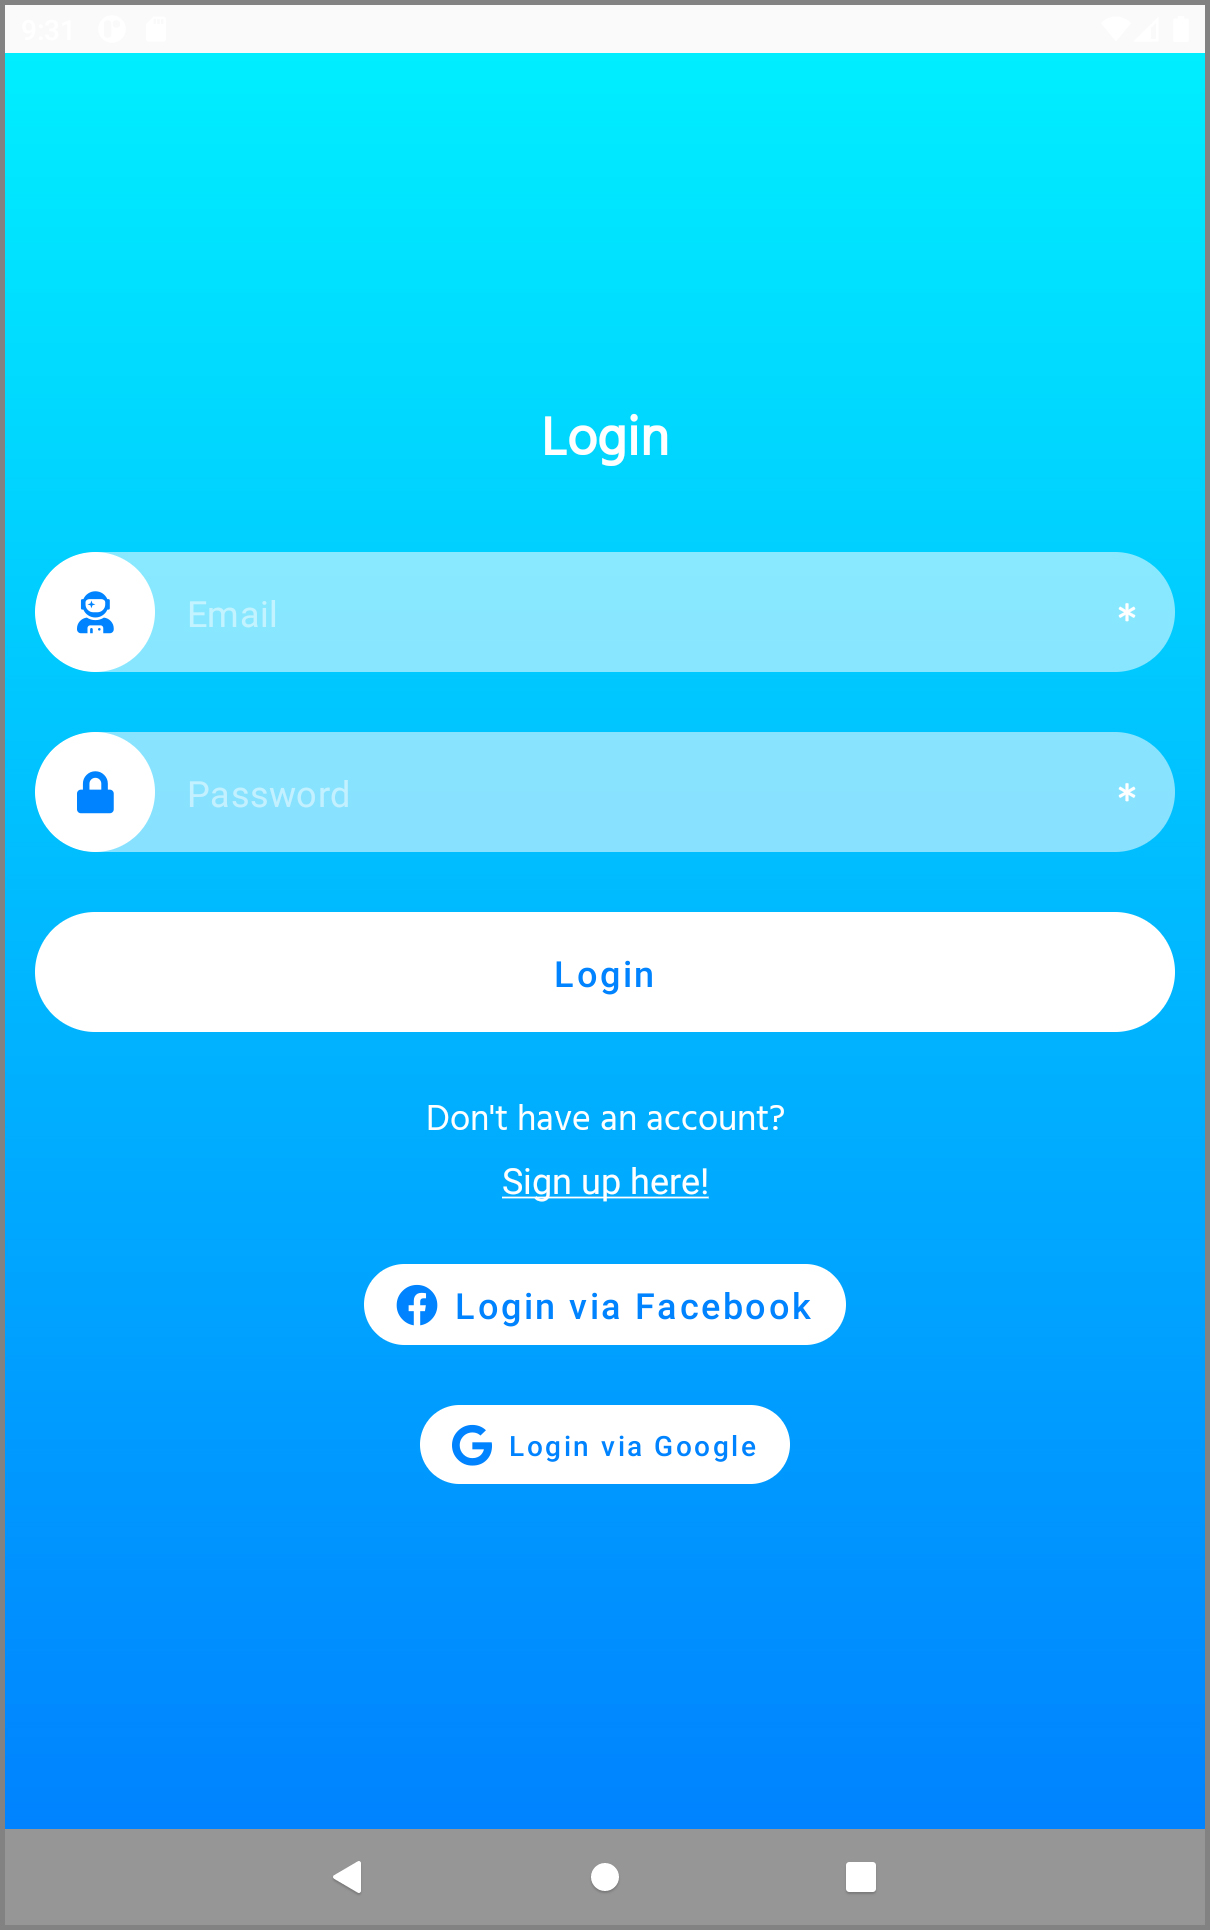
\includegraphics[width=.95\textwidth]{../Images/UI/LoginBig.jpg}
\caption{\label{fig:dbapiuser}\textbf{Login screen - Tablet}}
\end{minipage} 
\begin{minipage}{.45\textwidth}
\centering
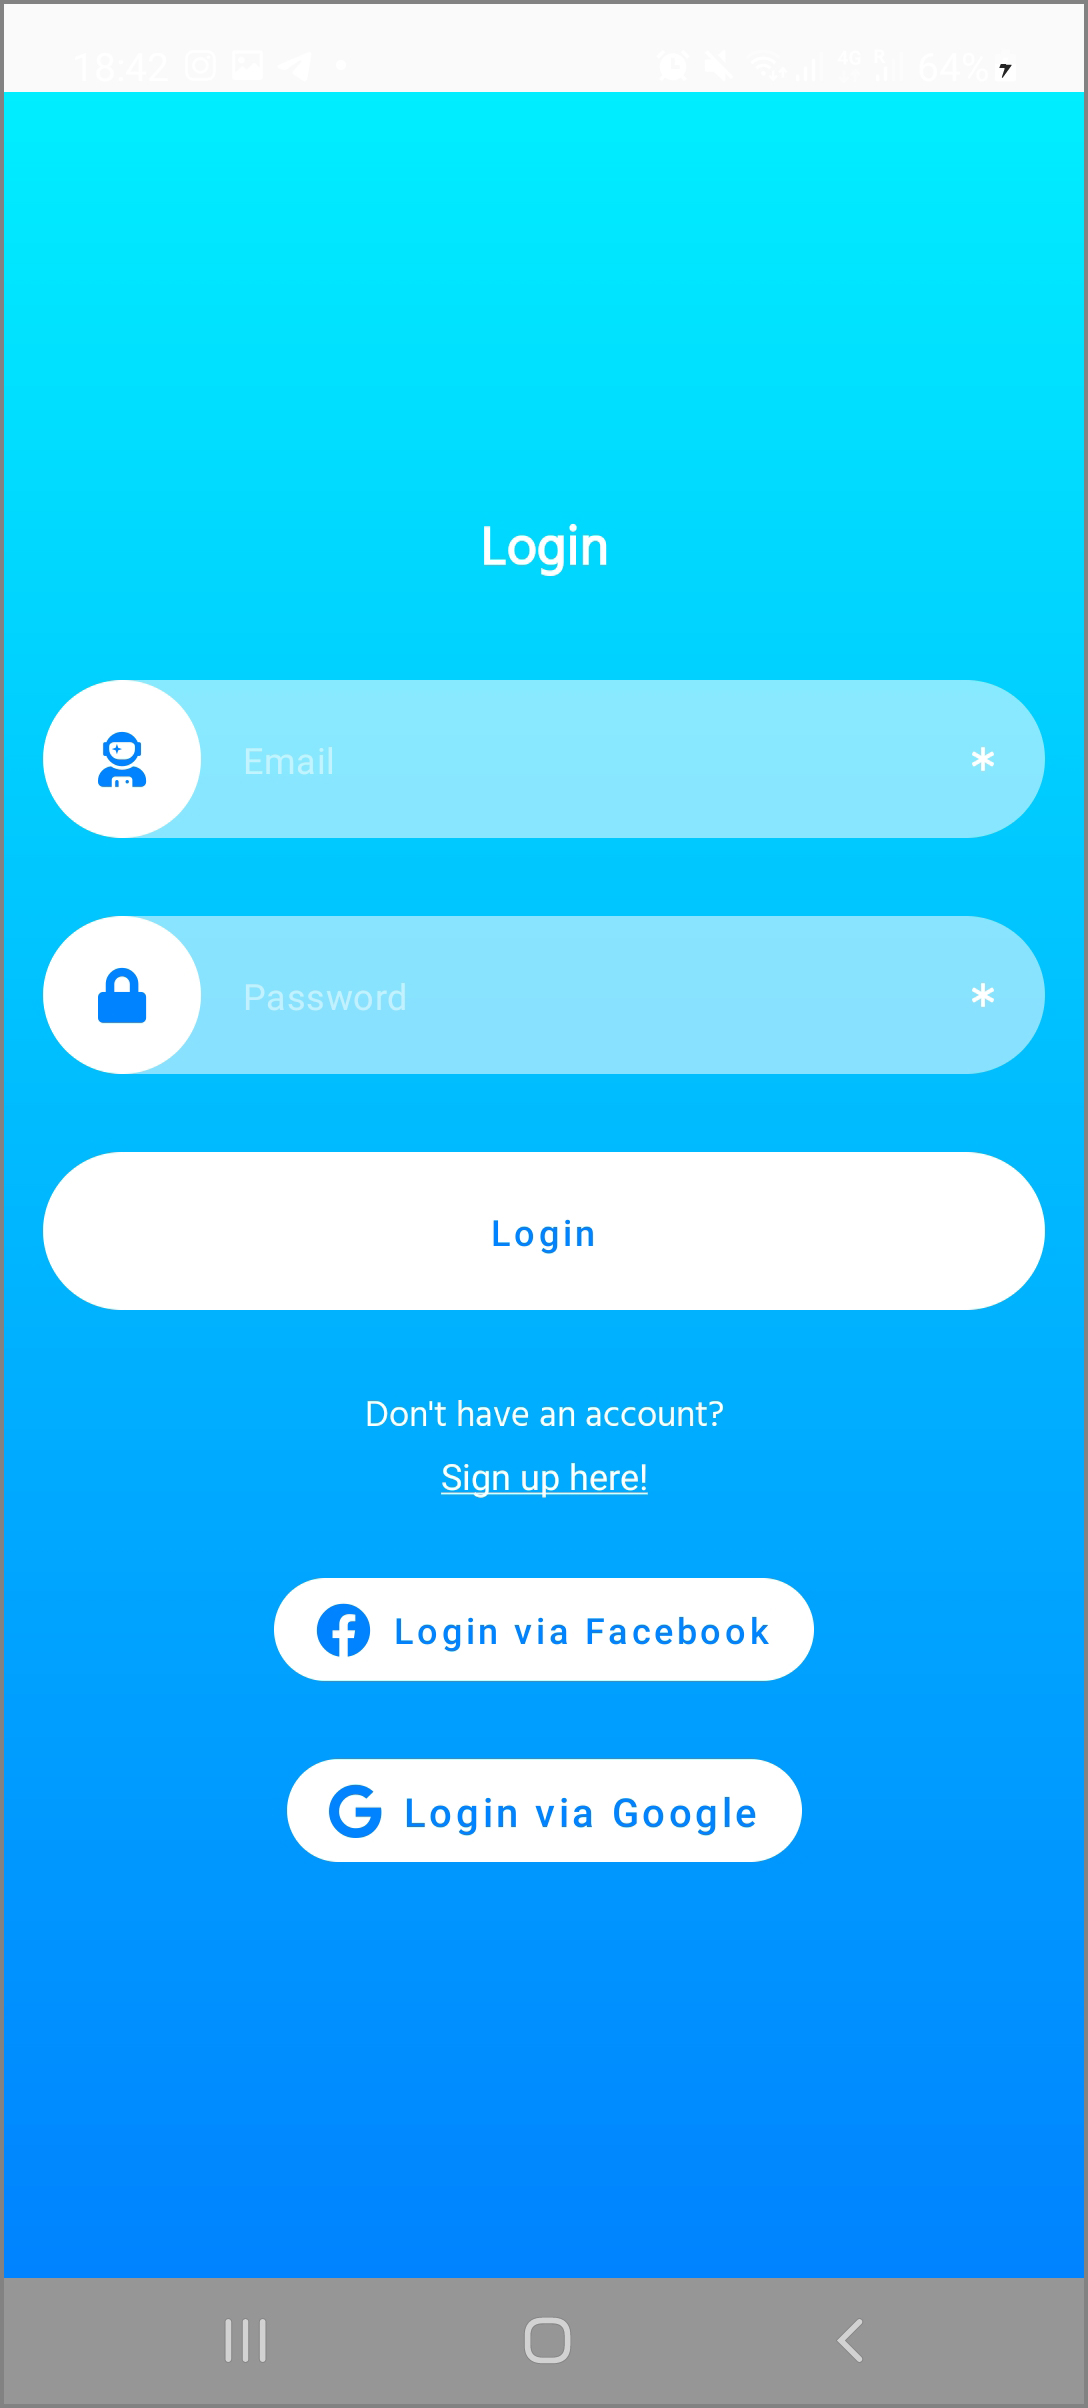
\includegraphics[width=.8\textwidth]{../Images/UI/Login.jpg}
\caption{\label{fig:dbapiuser}\textbf{Login screen - Phone}}
\end{minipage}
\end{figure}
 
\begin{figure}[!htb]
\centering
\begin{minipage}{.45\textwidth}
\centering
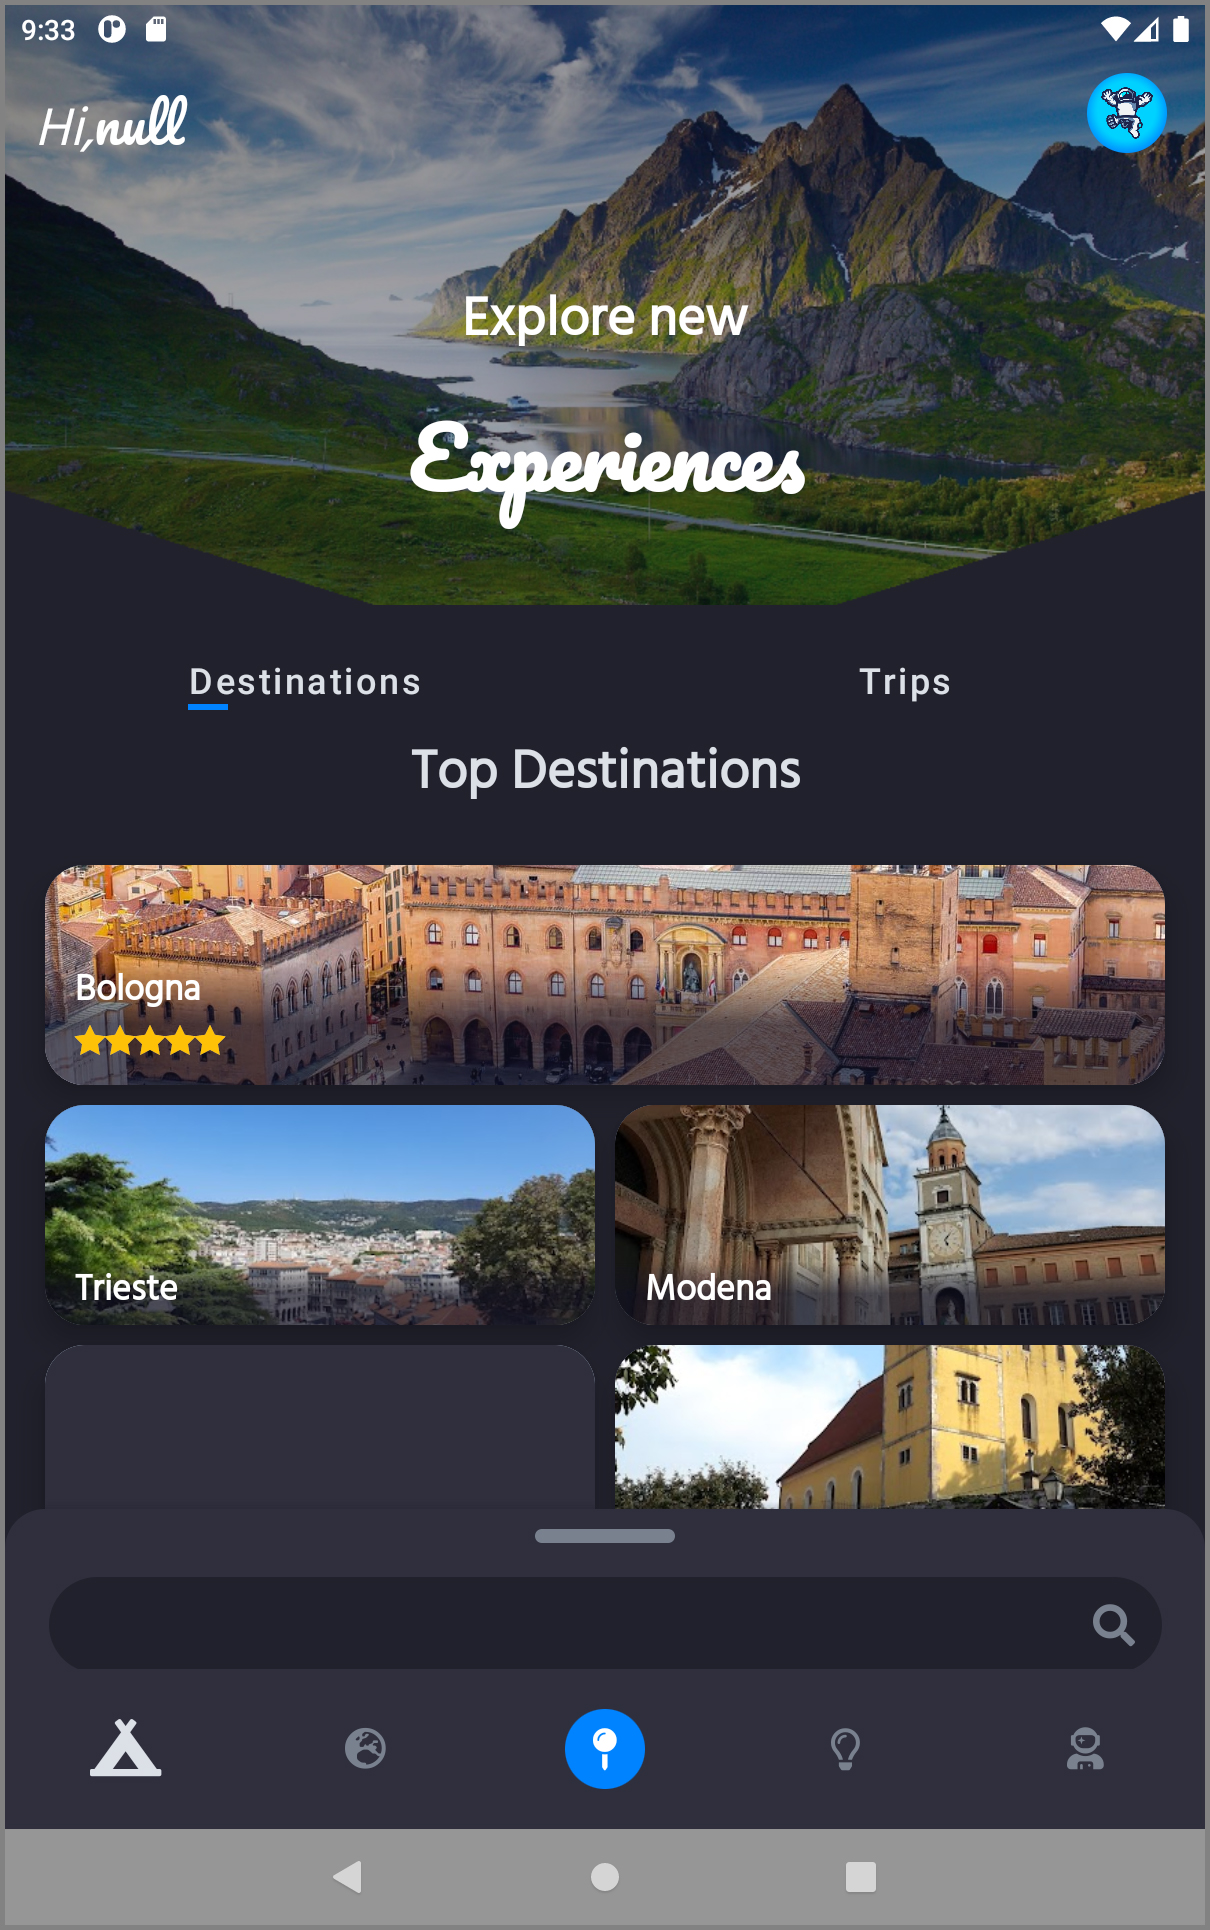
\includegraphics[width=.95\textwidth]{../Images/UI/HomeBig.jpg}
\caption{\label{fig:dbapiuser}\textbf{Home screen - Tablet}}
\end{minipage} 
\begin{minipage}{.45\textwidth}
\centering
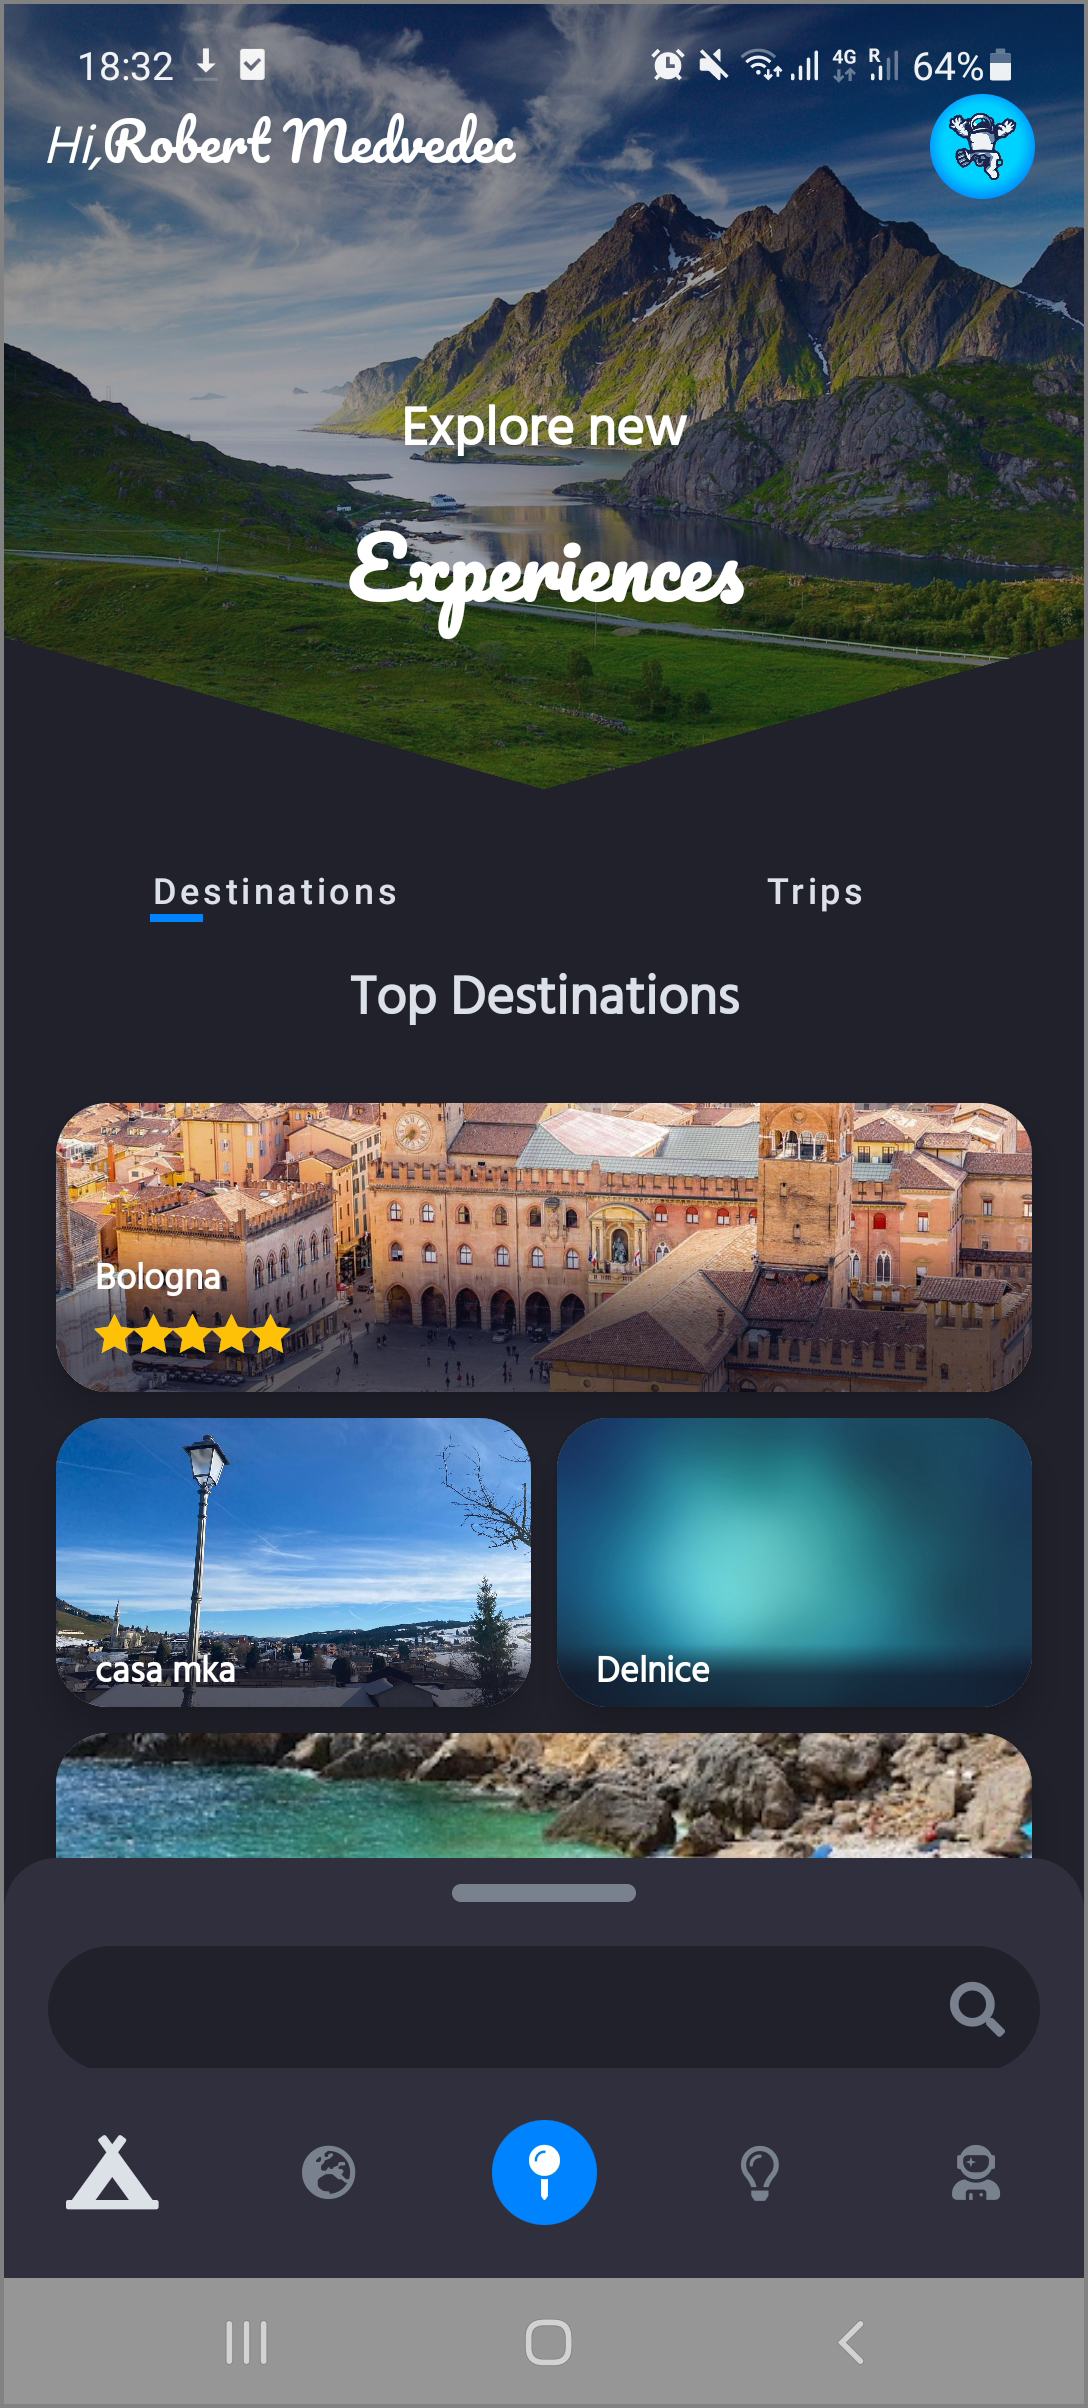
\includegraphics[width=.8\textwidth]{../Images/UI/DestinationsMain.jpg}
\caption{\label{fig:dbapiuser}\textbf{Home screen - phone}}
\end{minipage}
\end{figure} 

\begin{figure}[!htb]
\centering
\begin{minipage}{.45\textwidth}
\centering
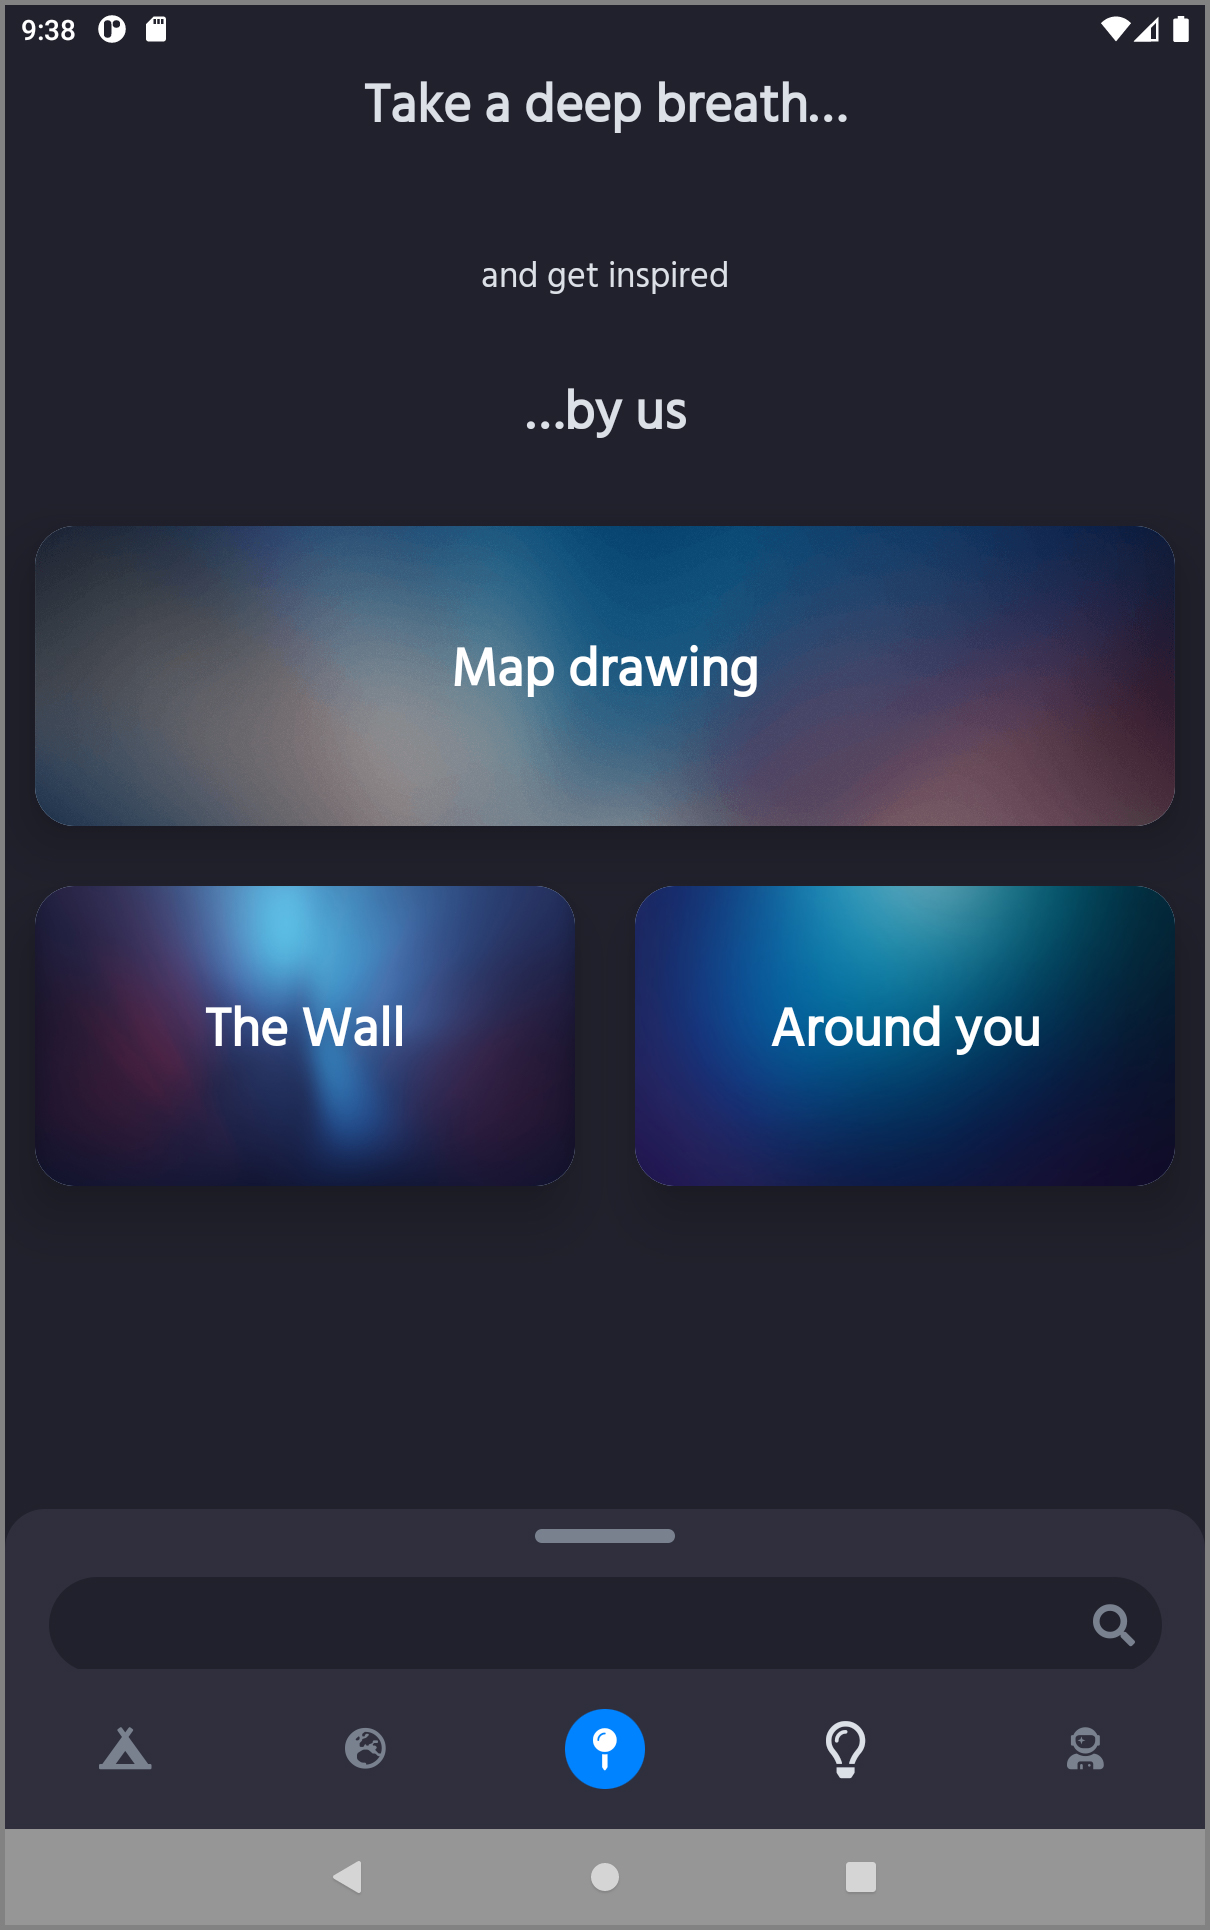
\includegraphics[width=.95\textwidth]{../Images/UI/ExploreBig.jpg}
\caption{\label{fig:dbapiuser}\textbf{Explore screen - Tablet}}
\end{minipage} 
\begin{minipage}{.45\textwidth}
\centering
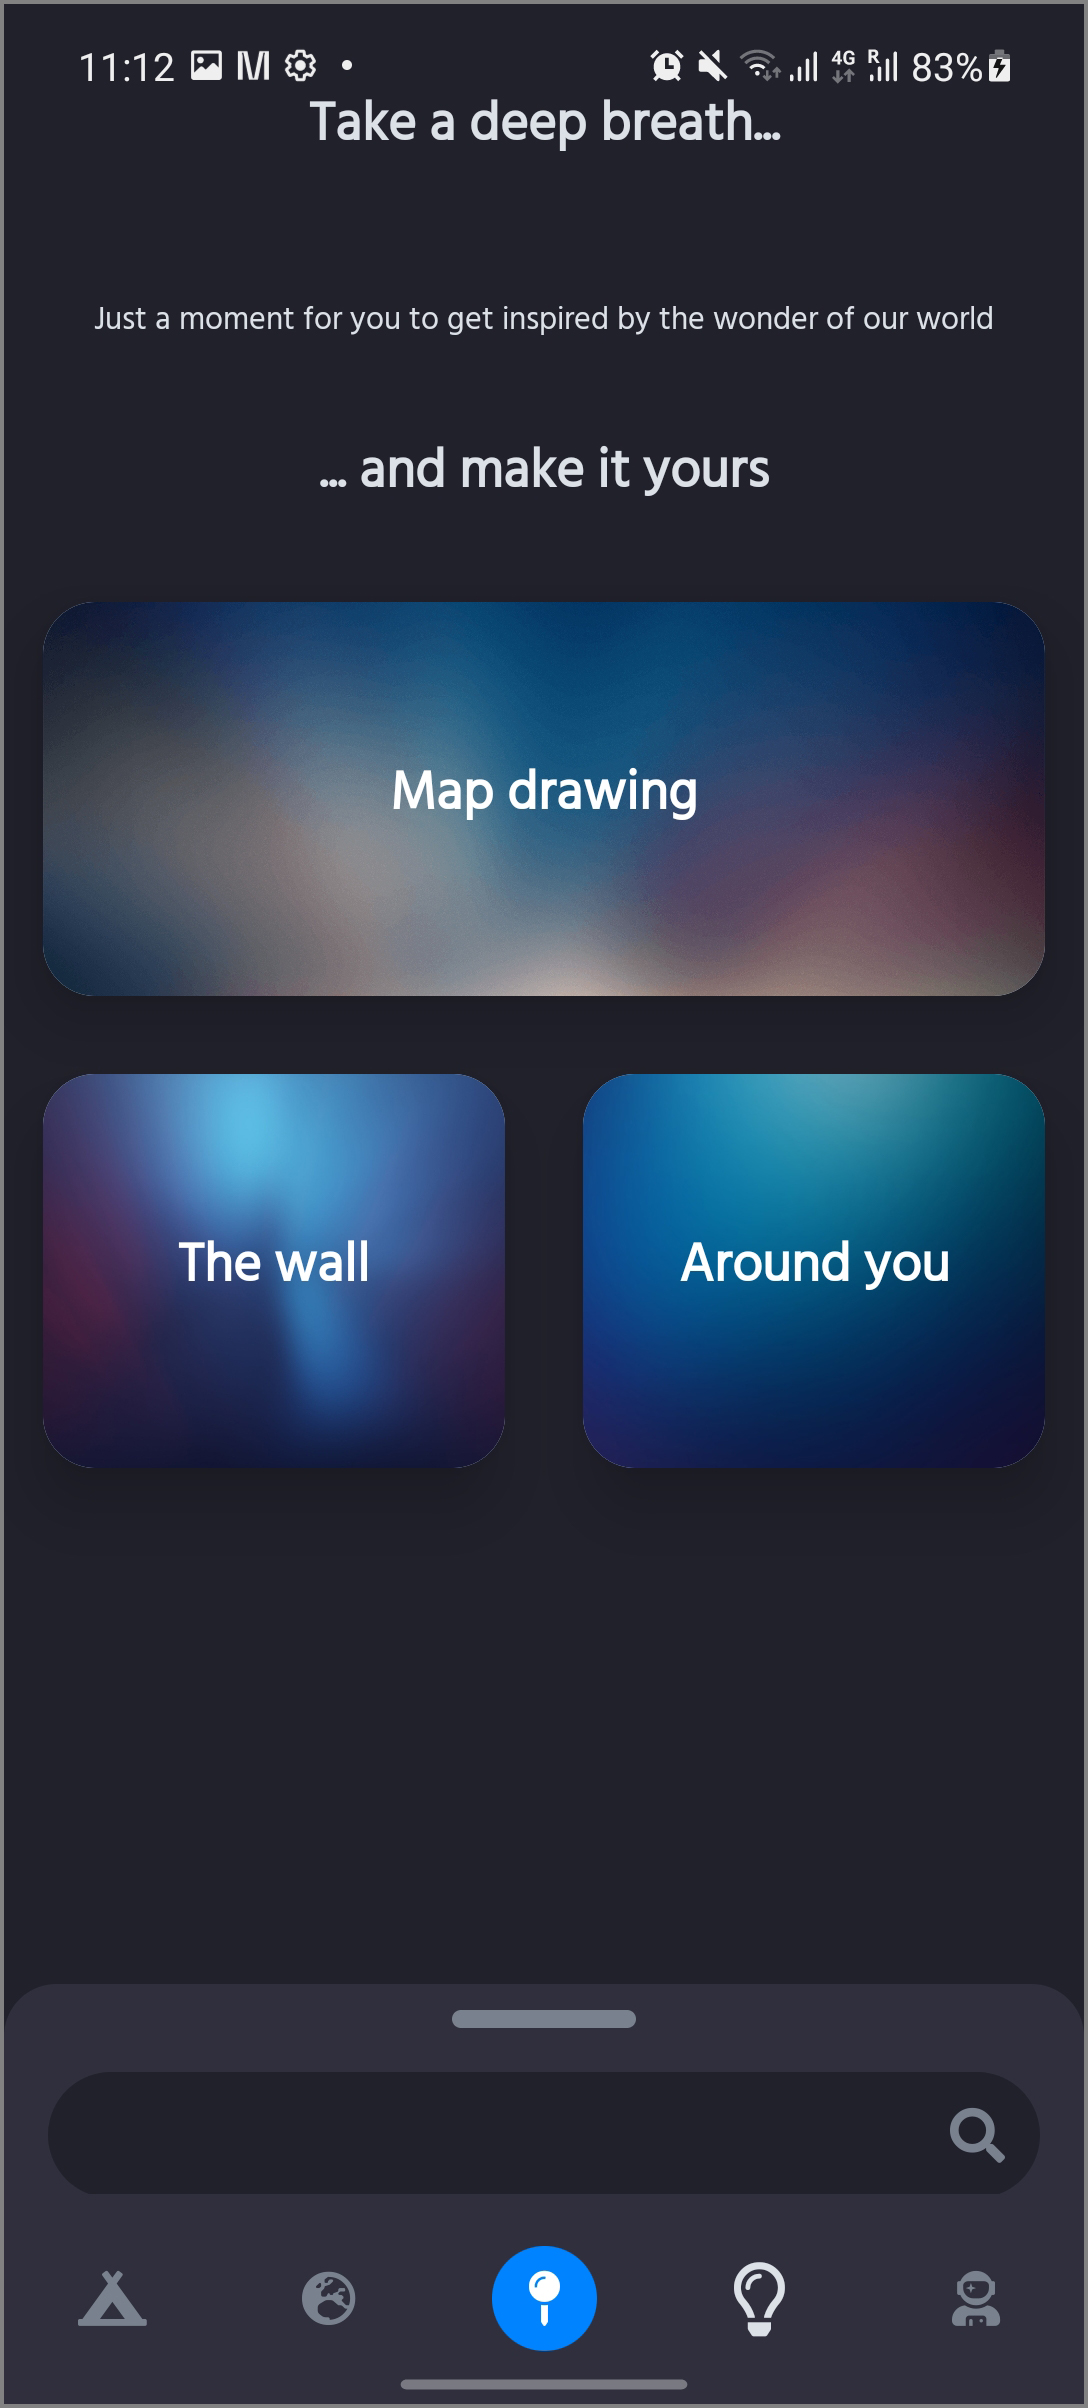
\includegraphics[width=.8\textwidth]{../Images/UI/ExploreDark.jpg}
\caption{\label{fig:dbapiuser}\textbf{Explore screen - Phone}}
\end{minipage}
\end{figure} 

\begin{figure}[!htb]
\centering
\begin{minipage}{.45\textwidth}
\centering
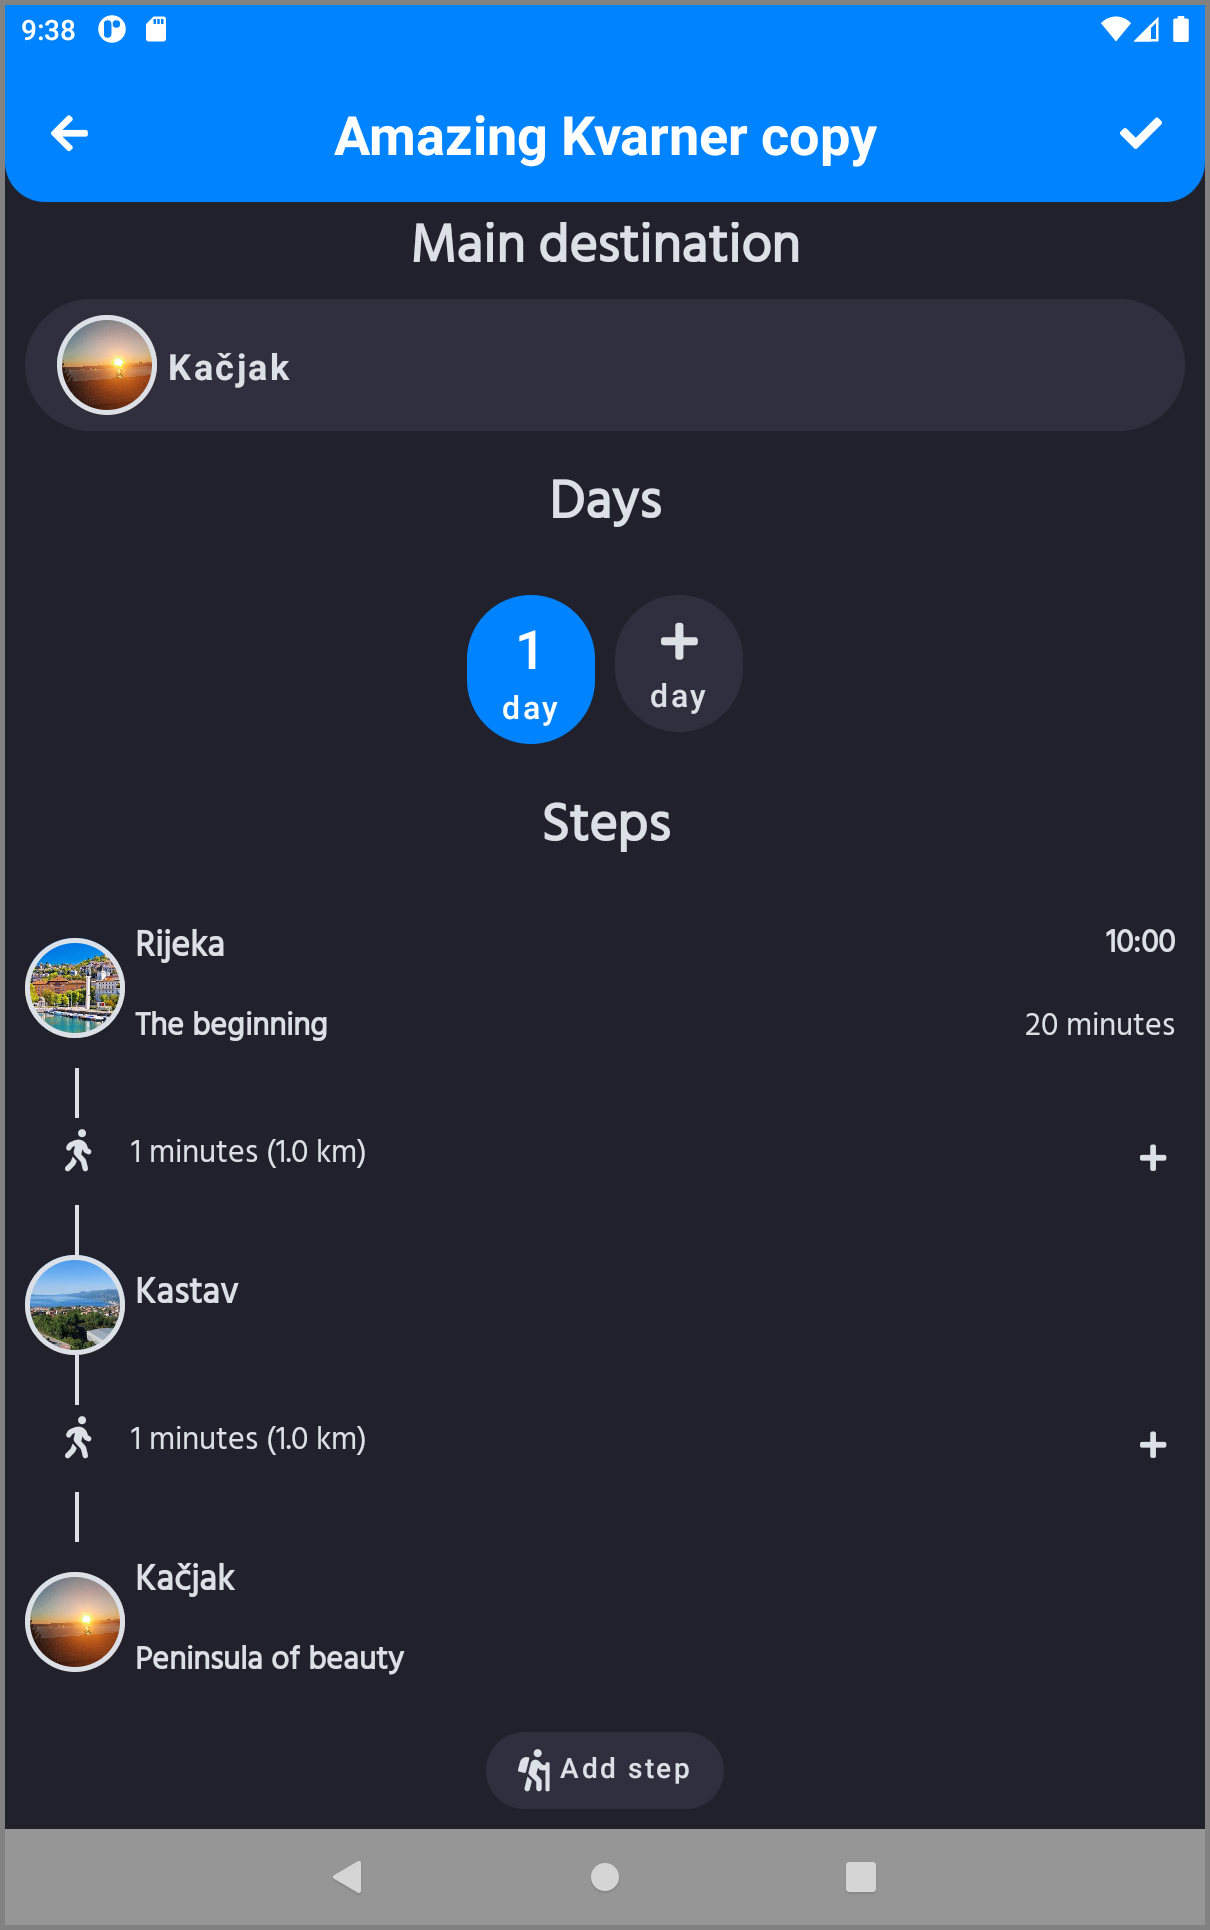
\includegraphics[width=.95\textwidth]{../Images/UI/TripCreateBig.jpg}
\caption{\label{fig:dbapiuser}\textbf{Trip create screen - Tablet}}
\end{minipage} 
\begin{minipage}{.45\textwidth}
\centering
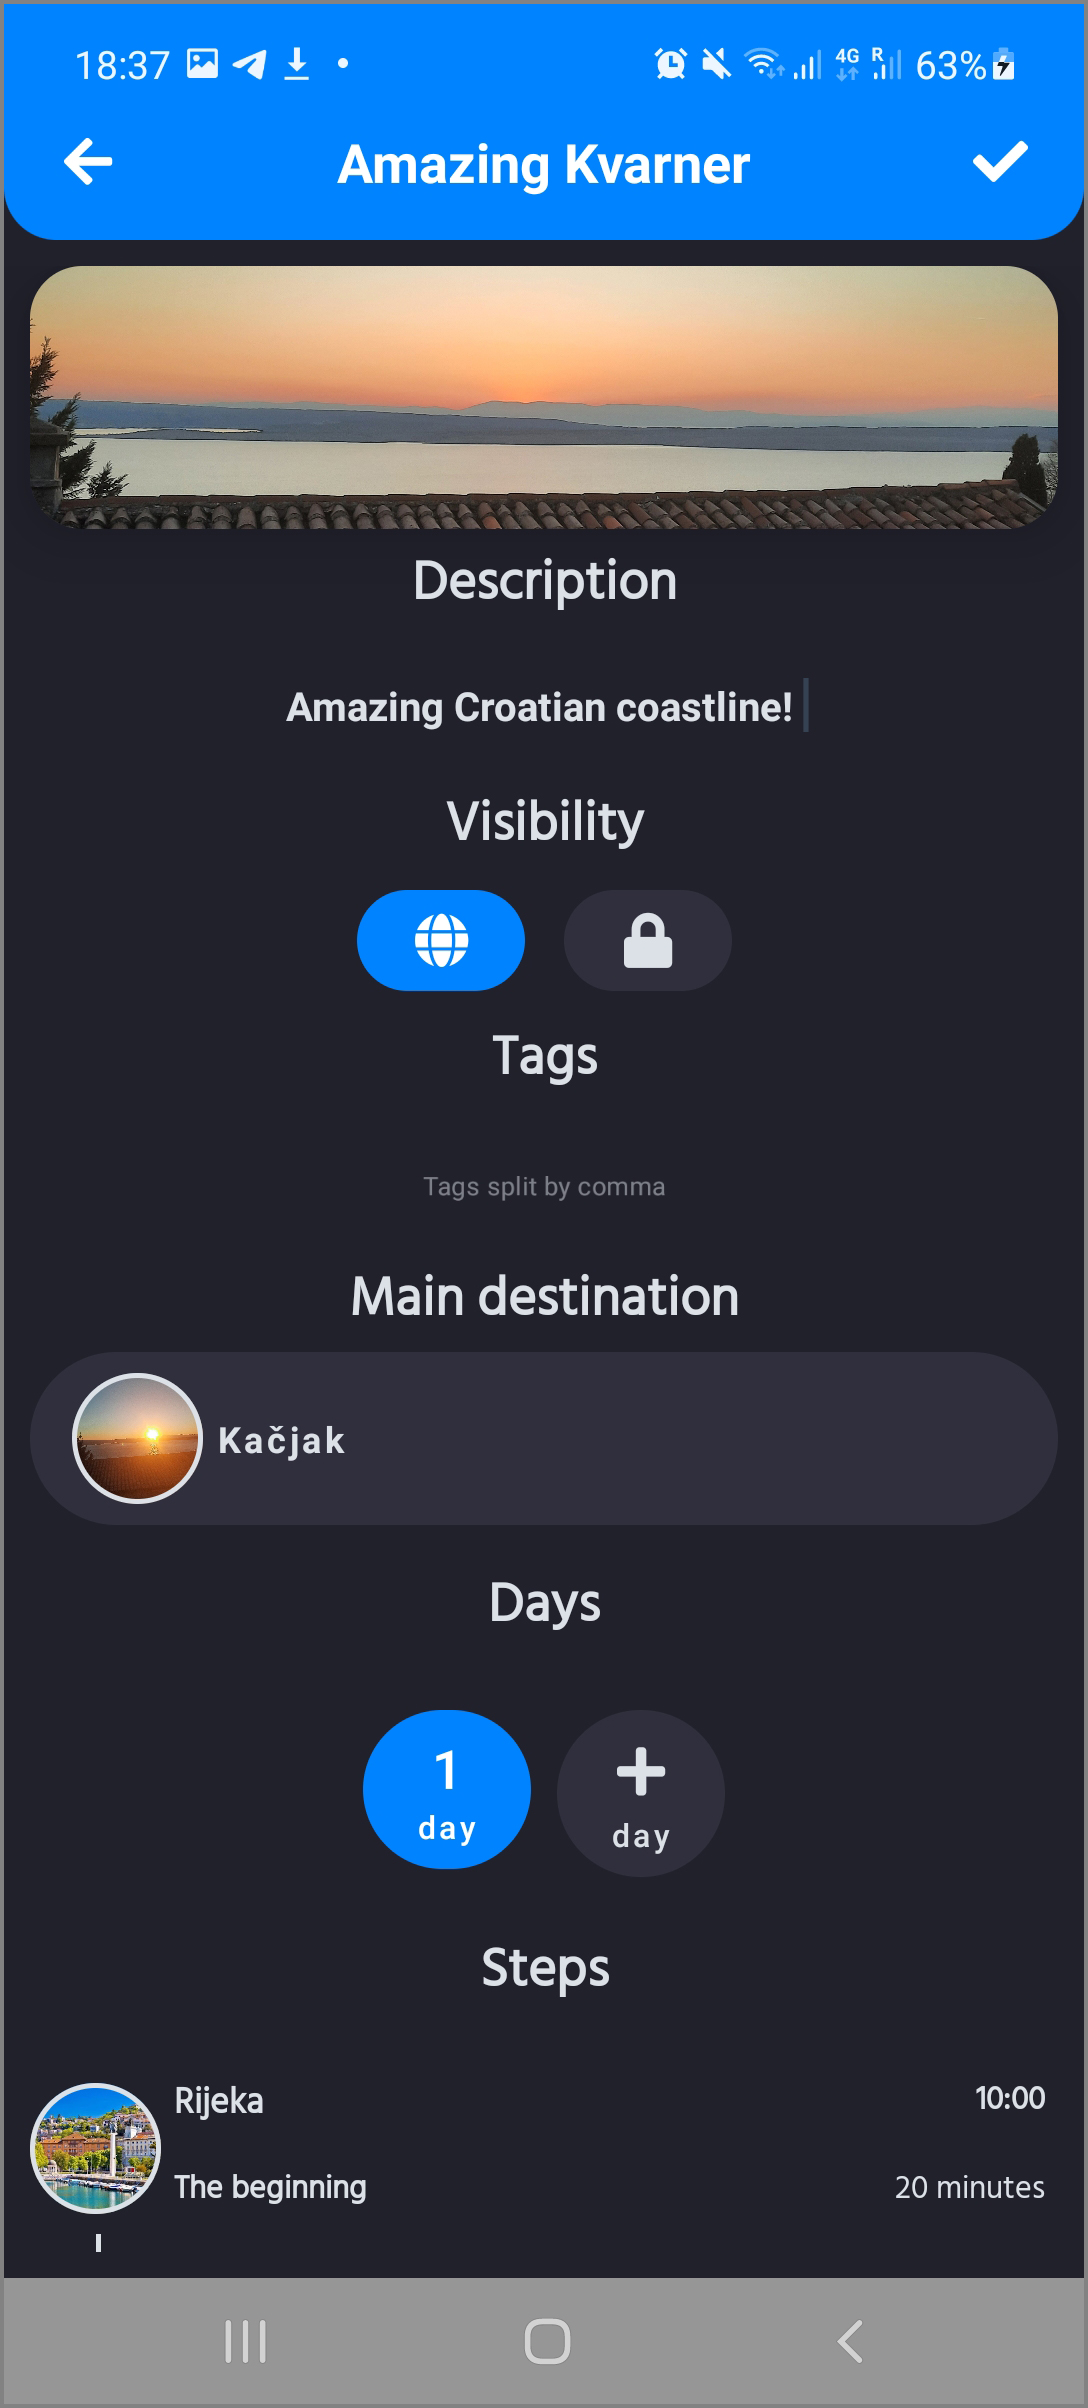
\includegraphics[width=.8\textwidth]{../Images/UI/TripCreateDark.jpg}
\caption{\label{fig:dbapiuser}\textbf{Trip create sreen - Phone}}
\end{minipage}
\end{figure} 

\newpage